\chapter{Introdução\label{chap:Introducao}}

O mercado global de animação e jogos foi avaliado em \$122.20 bilhões em 2010 e é esperado que esta cifra atinja  \$242.93 bilhões em 2016. Em relação ao mercado de animação, este pode ser dividido em Educação, Desenvolvimento para Web e Animação para Entretenimento, podendo esta última ser ainda subdividida em \textbf{Filmes} e \textbf{Efeitos Visuais}, dentre outras \cite{animationMarketSize}. Estas duas últimas categorias são de especial interesse para este trabalho. 

Uma tarefa recorrente dentro da indústria cinematográfica é a modelagem e animação de objetos tridimensionais. Tais objetos não estão sujeitos às restrições do mundo físico e permitem gerar cenas e movimentos dificilmente filmados de outra forma. Mesmo em produções com atores reais as técnicas de Animação Computacional se fazem presentes, seja transformando o cenário do filme, projetando sobre o ator uma textura que modifica suas feições ou adicionando à obra um personagem completamente digital. Presente em praticamente qualquer novo \textit{blockbuster}, as técnicas de animação tridimensional ainda apresentam custos elevados e proibitivos para certas aplicações.

O orçamento para a produção de um filme inclui custos de pré-produção, filmagem, pós-produção e divulgação, devendo-se acontar pelos direitos pelo roteiro, salários dos atores, salários da equipe de produção, construção do set de filmagens, efeitos especiais, figurino e tudo o mais \cite{movieProductionCost}. Apesar da Animação Computacional diminuir o custo de alguns dos componentes citados, ela é em si uma técnica cara. Ao passo que a animação computacional  reduz custos com montagem de cenários e até mesmo maquiagem, muitas vezes um único quadro de um filme pode requerer a animação milhões de partes móveis. Por exemplo, utilizaram-se mais de 2 milhões de fios de cabelo individualmente nomeados para a construção do personagem \textit{Sully} em \textit{Monstros SA (2011)}. Ainda neste filme, um único quadro com o personagem custou em média de 11 a 12 horas de trabalho criativo \cite{sullyExample}. Com tantas horas de trabalho criativo gastas durante o processo de animação, fica claro que é desejável o desenvolvimento de técnicas que auxiliem os animadores.

Uma técnica importante que vem ao auxílio dos animadores consistem em transferir movimentos e expressões de um ator para um modelo computacional. Metodologias para captura ótica de performance teatral capazes de registrar
expressões de um ator em geometria detalhada são utilizadas na indústria já há
algum tempo. Exemplo conhecido do uso desse tecnologia é o personagem \textit{Golum} no
filme \textit{O Senhor dos Anéis: A Sociedade do Anel } (2001), onde o ator Andy Serkis
utiliza um roupa especial com marcadores visuais durante as gravações para que
mais tarde a equipe de efeitos visuais renderize sobre ele um modelo
computacional tridimensional da criatura amaldiçoada. Mais recentemente, a mesma
tecnologia - em estado aprimorado e muito mais rica em detalhes - é utilizada em
\textit{O hobbit} (2015), onde o ator Benedict Cumberbatch dá vida ao dragão Smaug. A figura \ref{fig:smaug} ilustra o processo. Em \ref{fig:smaugA} vê-se o modelo que está sendo animado pela performance do ator. Em \ref{fig:smaugB} mostra-se em detalhes pontos colocados no rosto do ator para auxiliar a captura de expressões. 

\begin{figure*}[!htb]
   \centering
 \begin{subfigure}[]{\label{fig:smaugA}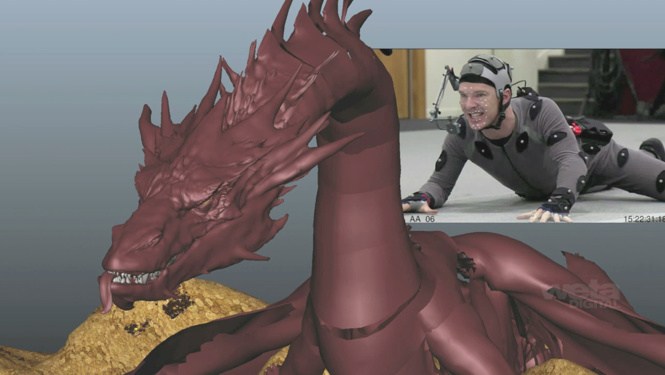
\includegraphics[width=0.4\linewidth]{./figs/exemploSmaug.jpg}}
  \end{subfigure}   
   \begin{subfigure}[]{\label{fig:smaugB}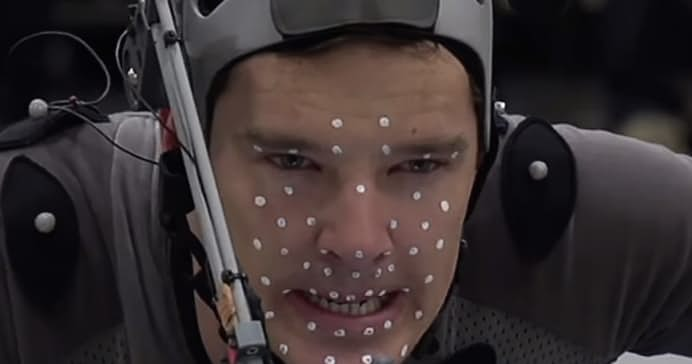
\includegraphics[width=0.4\linewidth]{./figs/Smaug_Benedict.jpg}}
  \end{subfigure}   
    \caption{Exemplo de utilização de captura de movimentos e expressões 
    na indústria cinematográfica. Pontos cuidadosamente colocados no rosto
  do ator são utilizados para transferir expressões para o modelo 
  tridimensional do personagem (retirado de \cite{sherlocksmaug}).}
    \label{fig:smaug}
\end{figure*}

Nesta aplicação cinematográfica requer-se do sistema de animação computacional uma alta precisão no
ajuste do modelo computacional ao ator em cena. Para esse fim, utilizam-se
ambientes especiais onde a iluminação é controlada, marcadores visuais são
utilizados no cenário e no ator e muitas vezes a captura da imagem é feita por
um arranjo de câmeras ou utiliza-se câmeras de alta resolução. Além disso, o resultado do processamento
recebe ainda um ajuste fino realizado por vários artistas para que resultado
apresentado seja o mais convincente possível. Vale notar que esse ajusto fino só
é possível pois há um longo prazo entre a captura da imagem e o instante em que
os resultados precisam ser apresentados ao público.

Outra aplicação para a animação auxiliada por captura de vídeo, desta vez com
requisitos de tempo muito mais severos, é o uso de fantoches digitais. Nesta
aplicação, vista em programas televisivos e em parques de diversão ao redor do
mundo, um ator em uma câmera escondida anima em tempo real um modelo renderizado
em projetor e responde ao vivo às perguntas do público. O personagem animado
apresenta expressões corporais e faciais que encantam o público, deixando os
mais novos convencidos de que conversaram com seu personagem preferido e os mais
velhos se perguntando como aquilo pode ser possível. Devido ao tempo de resposta
curto necessário para a interação entre público e personagem digital, não é
possível o ajusto fino dos artistas, mas ainda sim é possível fazer uso de
iluminação controlada, câmera(s) de alta qualidade e marcadores visuais. A
equipe por trás do personagem pode ainda fazer uso de controles pré-programados.

O problema com as configurações exigidas pelos produtos disponíveis atualmente é
o seu alto custo. Portanto, apesar de grandes empresas serem capazes de bancar o
preço da tecnologia atual, o surgimento de produtos que realizem as mesmas
tarefas a custos mais baixos é certamente de interesse do mercado. Tal produto
poderia, por exemplo, ser utilizado por animadores independentes para acelerar
seus projetos.

A aplicação que se tem em mente é justamente esta última. Programas de televisão
educacionais para crianças abundam no mercado, mas são em sua maioria
direcionadas ao público infantil geral. Um nicho de crianças não atendido é de
crianças autistas. Apesar de as dificuldades encontradas por estas crianças
variarem muito de um indivíduo para a outro, é comum que crianças autistas
apresentem dificuldade de manter contato visual, mesmo que seja com personagens
de um filme. Pretende-se que o produto desenvolvido neste trabalho seja
utilizado como ferramenta para auxiliar o desenvolvimento de programas infantis
com foco em crianças autistas.

O Capítulo 2 deste trabalho decorre sobre a fundamentação teórica 
por trás das técnicas utilizadas. Reconhecimento de pontos do rosto,
renderização de objetos tridimensionais, filtragem digital e estimação de
profundidade são tópicos abordados. No Capítulo 3 empregamos os conceitos
introduzidos no capítulo 3 e apresentamos a metodologia proposta para aplicação.
No Capítulo 4 apresentamos e discutimos os resultados obtidos. O último capítulo
elabora nossas conclusões e deixa propostas de melhorias futuras para o
trabalho.
